 \pstart [p.~21] Meae tamen eum tam fuse diducendi pepercissem operae, si quae doctissimus \textit{Maignanus}\protect\index{Namensregister}{\textso{Maignan,} Emanuel 1601\textendash 1671} hisce\footnote{\textit{Leibniz unterstreicht: Maignanus}\protect\index{Namensregister}{\textso{Maignan,} Emanuel 1601\textendash 1671} hisce} conformia, luculentius quidem opinor et accuratius, pertractavit, priusquam haec aggrederer contigisset inspexisse; [...] illius saltem eruditissimi viri\footnote{\textit{Hierzu am Rand}: Snellii\protect\index{Namensregister}{\textso{Snell van Royen} (Snellius), Willebrord 1580\textendash 1625} imo non consentit his. Confer hic pag. 37.} nefas fuerit non astipulari penitus, et acquiescere decreto; ''qui,
 \pend 
 \newpage 
 \pstart \noindent Deum unicum et Optimum Naturae Architectum, hanc (ait) legem radiis\protect\index{Sachverzeichnis}{lex!radiis} diversa media permeantibus praescripsisse; ut omnes omnino radii\protect\index{Sachverzeichnis}{radius} veri, et apparentes eandem semper inter se servent analogiam.''\footnote{\textit{Leibniz unterstreicht}: omnes [...] analogiam.\\ \textit{Hierzu am Rand die Zeichnung:}\\\protect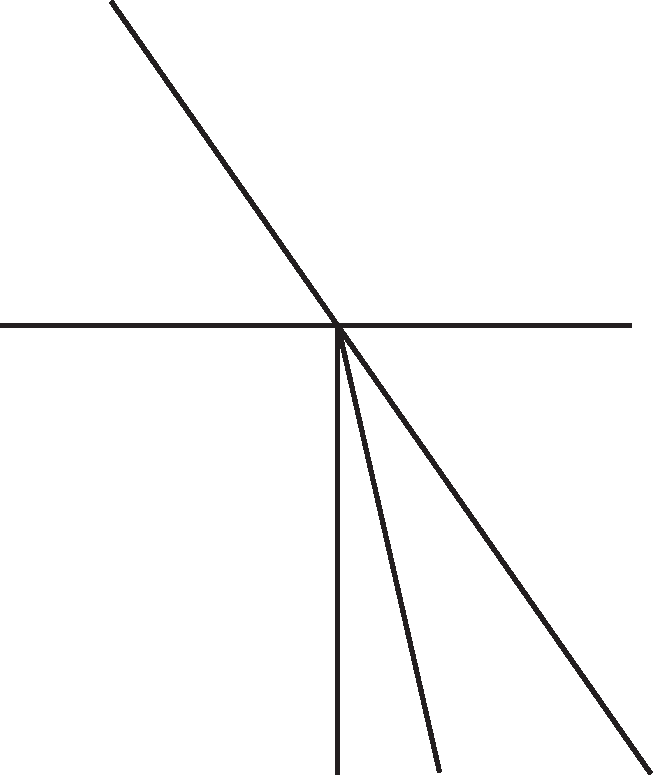
\includegraphics[width=0.1\textwidth]{images/Barrow_21}}\selectlanguage{latin}
 \pend